\section{Graphical user interface application} \label{sec:gui}
Within this section, I briefly overview the graphical user interface (GUI) application that allows to assemble and analyze complex networks of random variables graphically, without the need to specify such networks declaratory using the R, Python or even the C++ API. 

While the semantic of the \pkg{StochBB} API is closely related to the internal representation in terms of random variables, the GUI uses a more abstract representation. For example, models of cognitive processes are usually expressed in terms of a network of interacting \emph{processing stages}, each associated with a waiting time distribution. For the sake of simplicity, when analyzing such networks, the semantic of the network representation within the GUI is more related to \emph{processing stages} rather than random variables. 

All these \emph{processing stages} share the same form. They have at least one input socket that is the trigger of the stage and one output socket, that is the response. By chaining these stages, that is, connecting the output socket of one stage with the trigger socket of another stage, an equivalent of a sum of the waiting-time random variables of the chained stages is created. Although this representation is quiet uncommon in the field of statistics, it is very common in applied fields dealing with networks of random variables, like modeling of cognitive processes.

\begin{figure}[!ht]
 \centering
 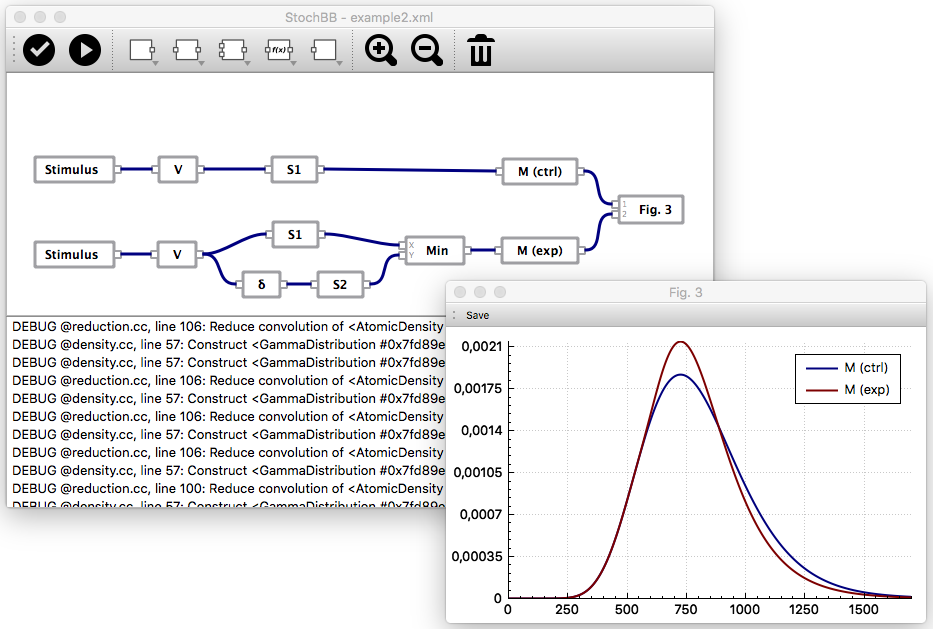
\includegraphics[width=.75\textwidth]{fig/GUI2.png}
 \caption{Overview of the GUI of \pkg{StochBB}, the toolbar at the top of the main window (background), network edit field in the middle of the main window, the log view at the bottom of the main window (can be hidden) and a separate plot window at the foreground.} \label{fig:gui}
\end{figure}

\subsection{General overview}
The main window of the GUI (see Figure \ref{fig:gui}) consists of two parts:
\begin{enumerate}
 \item The tool bar at the top of the main window. Here, frequently used actions are collected like verifying the network, performing the analysis,
 adding or removing items. All these actions are also available at the main menu (not shown in Fig. \ref{fig:gui}).
 \item The network view at the center of the main window. Here the network of \emph{stages} can be viewed and edited. This view is described in more detail below.
\end{enumerate}

Additionally, there  is a log window at the bottom. By default, this view is hidden and can be enabled at the menu under \emph{View} $\rightarrow$ \emph{Show log}. It displays various messages from the core library emitted during the verification and analysis of the network. 


\subsection{Editing a network}
Within the network view, the network is shown and can be assembled or modified. New items (e.g., stages) can be added to the network by selecting them from either the tool bar or from the menu under \emph{Edit} (see Figure \ref{fig:items} for some examples). These items can then be moved around in the network view by simply dragging them. An item can be removed by first selecting it with a single click and choosing \emph{Edit} $\rightarrow$ \emph{Remove} from the main menu or the \emph{Remove} button in the tool bar.

All network items have at least two properties that can be edited by double-clicking the item. Its label, shown inside the box representing the item in the network view, and a descriptive text (not shown) that allows to document the item. Many nodes, particularly those representing \emph{stages} with some parametric waiting-time distribution, have additional parameters that specify the waiting-time distribution. 

\begin{figure}[!ht]
 \begin{subfigure}[c]{0.2\textwidth}
   \centering
 	
\includegraphics[width=0.8\textwidth]{fig/guitrigger.pdf}
 	\caption{Trigger/Stimulus item.} \label{fig:itemtrigger}
 \end{subfigure}\hfill
 \begin{subfigure}[c]{0.2\textwidth}
   \centering
 	
\includegraphics[width=0.45\textwidth]{fig/guigamma.pdf}
 	\caption{Gamma distr. random variable.} \label{fig:itemgamma}
 \end{subfigure}\hfill
 \begin{subfigure}[c]{0.2\textwidth}
   \centering
 	
\includegraphics[width=0.65\textwidth]{fig/guigammac.pdf}
 	\caption{Compound Gamma distr. random variable.} \label{fig:itemgammac}
 \end{subfigure} \hfill
 \begin{subfigure}[c]{0.2\textwidth}
   \centering
 	
\includegraphics[width=0.6\textwidth]{fig/guigammap.pdf}
 	\caption{Gamma distr. stage.} \label{fig:itemgammap}
 \end{subfigure}
 
 \begin{subfigure}[c]{0.2\textwidth}
   \centering
 	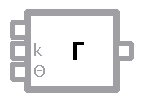
\includegraphics[width=0.6\textwidth]{fig/guigammacp.pdf}
 	\caption{Compound Gamma distr. stage.} \label{fig:itemgammacp}
 \end{subfigure}\hfill
 \begin{subfigure}[c]{0.2\textwidth}
   \centering
 	
\includegraphics[width=0.8\textwidth]{fig/guimin.pdf}
 	\caption{Minimum stage.} \label{fig:itemmin}
 \end{subfigure}\hfill
 \begin{subfigure}[c]{0.45\textwidth}
   \centering
 	
\includegraphics[width=0.8\textwidth]{fig/guiinh.pdf}
 	\caption{Inhibition stage.} \label{fig:iteminh}
 \end{subfigure}
 
  \begin{subfigure}[c]{0.4\textwidth}
    \centering
 	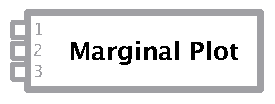
\includegraphics[width=0.6\textwidth]{fig/guiplot.pdf}
 	\caption{Marginal plot.} \label{fig:itemplot}
 \end{subfigure}\hfill
  \begin{subfigure}[c]{0.4\textwidth}
    \centering
 	
\includegraphics[width=0.55\textwidth]{fig/guiscatter.pdf}
 	\caption{Scatter plot.} \label{fig:itemscatter}
 \end{subfigure}
 \caption{Some examples of stages available in the GUI application.} \label{fig:items}
\end{figure}

All networks items have so-called sockets (small rectangles at the left or right side of the item, compare Fig. \ref{fig:items}). These sockets can be used to connect the items to form a network. All sockets on the left side of an item are input sockets and all on the right are outputs. Although a single output socket might be connected to several input sockets, every input can only be connected to single output socket. Like with network items, a connection can be removed by selecting it with a single click and choosing \emph{Edit} $\rightarrow$ \emph{Remove} from the main menu or the \emph{Remove} button in the tool bar.

All items can be divided into five groups: \emph{Random variables}, \emph{random stages}, \emph{join stages}, \emph{transformations} and \emph{plots}. \emph{Random variable} items (e.g., Figs. \ref{fig:itemtrigger}-\ref{fig:itemgammac}) represent simple random variables with some parametric distribution, which usually (except for compound random variables, e.g., Fig. \ref{fig:itemgammac}) have no input slots. One special item is the trigger or stimulus item (see Fig. \ref{fig:itemtrigger}). Although being a simple random variable with some $\delta$~distribution, that is a constant, it is ment to specify an event at a fixed time-point. There can be an arbitrary number of trigger items in every network (e.g. a stimulus at $T=0$ and a second manipulation of the experiment at some later time point).

All items of the \emph{random stage} group (e.g., Figs. \ref{fig:itemgammap}, \ref{fig:itemgammacp}) have a trigger input socket. Although being similar to the \emph{random variable} items, they might be considered as \emph{processing stages} with some parametric waiting-time distribution. That is, its output is a random variable being the sum of its input and a random variable distributed according to some parametric distribution. Like for the simple \emph{random variable} items, there are also \emph{random stage} items with a compound waiting-time distribution (e.g., Fig. \ref{fig:itemgammacp}).

As mentioned above, an input socket may only be connected to a single output socket, although a single output may be connected to several inputs. This is due to the fact, that the function for joining several \emph{signal paths} must be specified explicit. \emph{Join stages} (see Figs. \ref{fig:itemmin}, \ref{fig:iteminh}) are these functions that can be used to join signal paths according to some function. 

For example the \emph{minimum} stage (Fig. \ref{fig:itemmin}) represents the minimum of the inputs $X$ and $Y$. Or, in terms of processing stages, it gets triggered once either the stage connected to the $X$ input or the stage connected to the $Y$ input completed. A special \emph{join stage} is the \emph{inhibition} stage (Fig. \ref{fig:iteminh}). It represents the \emph{conditional sum} random variable introduced above and is the only stage represented by two items. The first item labeled \emph{inh} forwards the first event and inhibits the second. For example, it triggers only the stages connected to the $X$ output socket if the stage connected to the $X$ input completes first. The second item labeled \emph{join} then joins the two mutually exclusive signal paths into one. The \emph{conditional} random variable introduced above, is not included as a \emph{random stage} item as it would break causality.

Finally, the \emph{plot} items (see Figs. \ref{fig:itemplot}, \ref{fig:itemscatter}) allow for evaluating or sampling from the network. When added to the network, the \emph{Marginal Plot} item (Fig. \ref{fig:itemplot}) has no inputs at all. This item has a \emph{graphs} property that defines the number of graphs and consequently the number of inputs for this item. After this property has been set to the desired value, the corresponding number of inputs will appear at the item. In contrast, the \emph{Scatter Plot} item has always two inputs. They specify the two random variables to sample from for a scatter plot.

\subsection{Verifying the network and running an analysis}
Performing an analysis consists of two steps. In a first step, a network of random variables is derived from the stage-network representation used by the GUI application. This step will fail if any assumption (e.g., independence assumptions) made by the derived random variables is not met. This step will fail too, if there is a cyclic dependency between stages or an unconnected input socket. Once the network of random variables is derived, it is ensured that the network is consistent. Hence running an analysis and verifying the network share this first step. 

In a second step, the derived network of random variables is actually analyzed. That is, the marginal distributions of the random variables being plotted are obtained and evaluated on the desired intervals. For the \emph{Scatter plots} or \emph{KDE plots}, a sampler gets instantiated to obtain samples from the random variables of interest. Finally, the plots are created and shown in separate plot windows.